\lstinputlisting[language=bash,basicstyle=\small]{python_codes/fieldstone_68/keywords.ascii}

\begin{center}
Code at \url{https://github.com/cedrict/fieldstone/tree/master/python_codes/fieldstone_68}
\end{center}

\par\noindent\rule{\textwidth}{0.4pt}

{\sl This fieldstone was developed in collaboration with Iris van Zelst}. \index{contributors}{I. van Zelst}

\par\noindent\rule{\textwidth}{0.4pt}

%%%%%%%%%%%%%%%%%%%%%%%%%%%%%%%%%%%%%%%%%%%%%%%%%%%%%%%%%%%%%%%%%%%%%%%%%%%%%%%%%%%%%%%%%%%%%%%%%%%%


\Literature: \\
\textcite{vack08}\citetitle{vack08}\\
\textcite{syva10}\citetitle{syva10}\\
\textcite{vakn12}\citetitle{vakn12}\\
\textcite{vaws19}\citetitle{vaws19}\\
\textcite{enma21}\citetitle{enma21}\\
\textcite{gadm22}\citetitle{gadm22}

%------------------------------------------------------------
\subsubsection*{Description of the setup and benchmark cases}


The domain is $660\text{km}\times 600\text{km}$. 

\begin{center}
\includegraphics[width=14cm]{python_codes/fieldstone_68/images/fig1}\\
{\captionfont Taken from van Keken et al (2008) \cite{vack08}.
(a) Cartoon of the cornerflow model for subduction zone dynamics. 
(b) Benchmark geometry of a kinematic slab driving flow in the viscous
mantle wedge below a rigid overriding plate. 
(c) Boundary conditions for Stokes and temperature equations.}
\end{center}

As shown in the figure above, 
the inflow boundaries (at both wedge and trench sides) and top of the model 
have prescribed temperature. The wedge is assumed to be an incompressible fluid that
is driven only by the kinematic forcing of the slab. The wedge is
confined by the top of the slab and the base of the rigid overriding
plate (located at a depth of $50\text{km}$). 
The boundary conditions for the wedge are no-slip below the overriding plate and constant velocity
along the top of the slab. The velocity boundary conditions for the
boundaries of the wedge are either provided by the Batchelor cornerflow 
solution (cases 1a and 1b) or based on free inflow/outflow
boundaries (cases 1c, 2a, 2b). The velocity field is discontinuous between the slab
and the overriding plate.
The velocity in the slab is constant (5cm/yr) and it dips at a $45\degree$ angle
There is no radiogenic of shear heating.
The mantle wedge rheology is either linear viscous (cases 1a,b,c),
diffusion creep (case 2a) or dislocation creep (case 2b).





%___________________
\paragraph{Case 1a} The Stokes equations are not solved. Instead the velocity field
is prescribed analytically everywhere in the domain, using the corner flow solution 
in the mantle wedge. 

%___________________
\paragraph{Case 1b - dynamical flow in isoviscous wedge I}
This case is the same as 1a, except that the solution
for the wedge flow is determined by solving the Stokes equations while the Batchelor solution is
imposed on the inflow and outflow boundaries. This case tests the ability of the numerical method
to accurately reproduce the corner flow solution.

%___________________
\paragraph{Case 1c - dynamical flow in isoviscous wedge II} 
Same as case 1b, but with stress-free boundary conditions on the mantle wedge.

%___________________
\paragraph{Case 2a}

This case is the same as 1c, except that the viscosity of the wedge
is given by 
\[
\eta_{\text{diff,eff}} = \left( \frac{1}{\eta_{\text{diff}}} + \frac{1}{\eta_{\text{max}}} \right)^{-1}
\]
and
\[
\eta_{\text{diff}}=A_{\text{diff}} \exp\left( \frac{Q_{\text{diff}}}{RT} \right)
\]
with
$Q_{diff}=335kJ/mol$ and $A_{diff}=1.32043 \cdot 10^9Pa\cdot s$. $\eta_{max}=10^{26}$Pa.s

%___________________
\paragraph{Case 2b}

This case is the same as 1c, except that the viscosity of the wedge
is given by 
\[
\eta_{\text{disl,eff}} = \left( \frac{1}{\eta_{\text{disl}}} + \frac{1}{\eta_{\text{max}}} \right)^{-1}
\]
and
\[
\eta_{\text{disl}}=
A_{\text{disl}} \dot\varepsilon^{(1-n)/n} \exp \left( \frac{Q_{\text{disl}}}{nRT} \right)
\]
with $Q_{\text{disl}}=540kJ/mol$, $n=3.5$ and $A_{\text{disl}}=28968.6Pa\cdot s^{1/n}$. 
$\eta_{\text{max}}=10^{26}$Pa.s


%------------------------------------------------------------
\subsubsection*{Mesh and boundary conditions}

The mesh is composed of square elements which are subdivided in two, as shown here:

\begin{center}
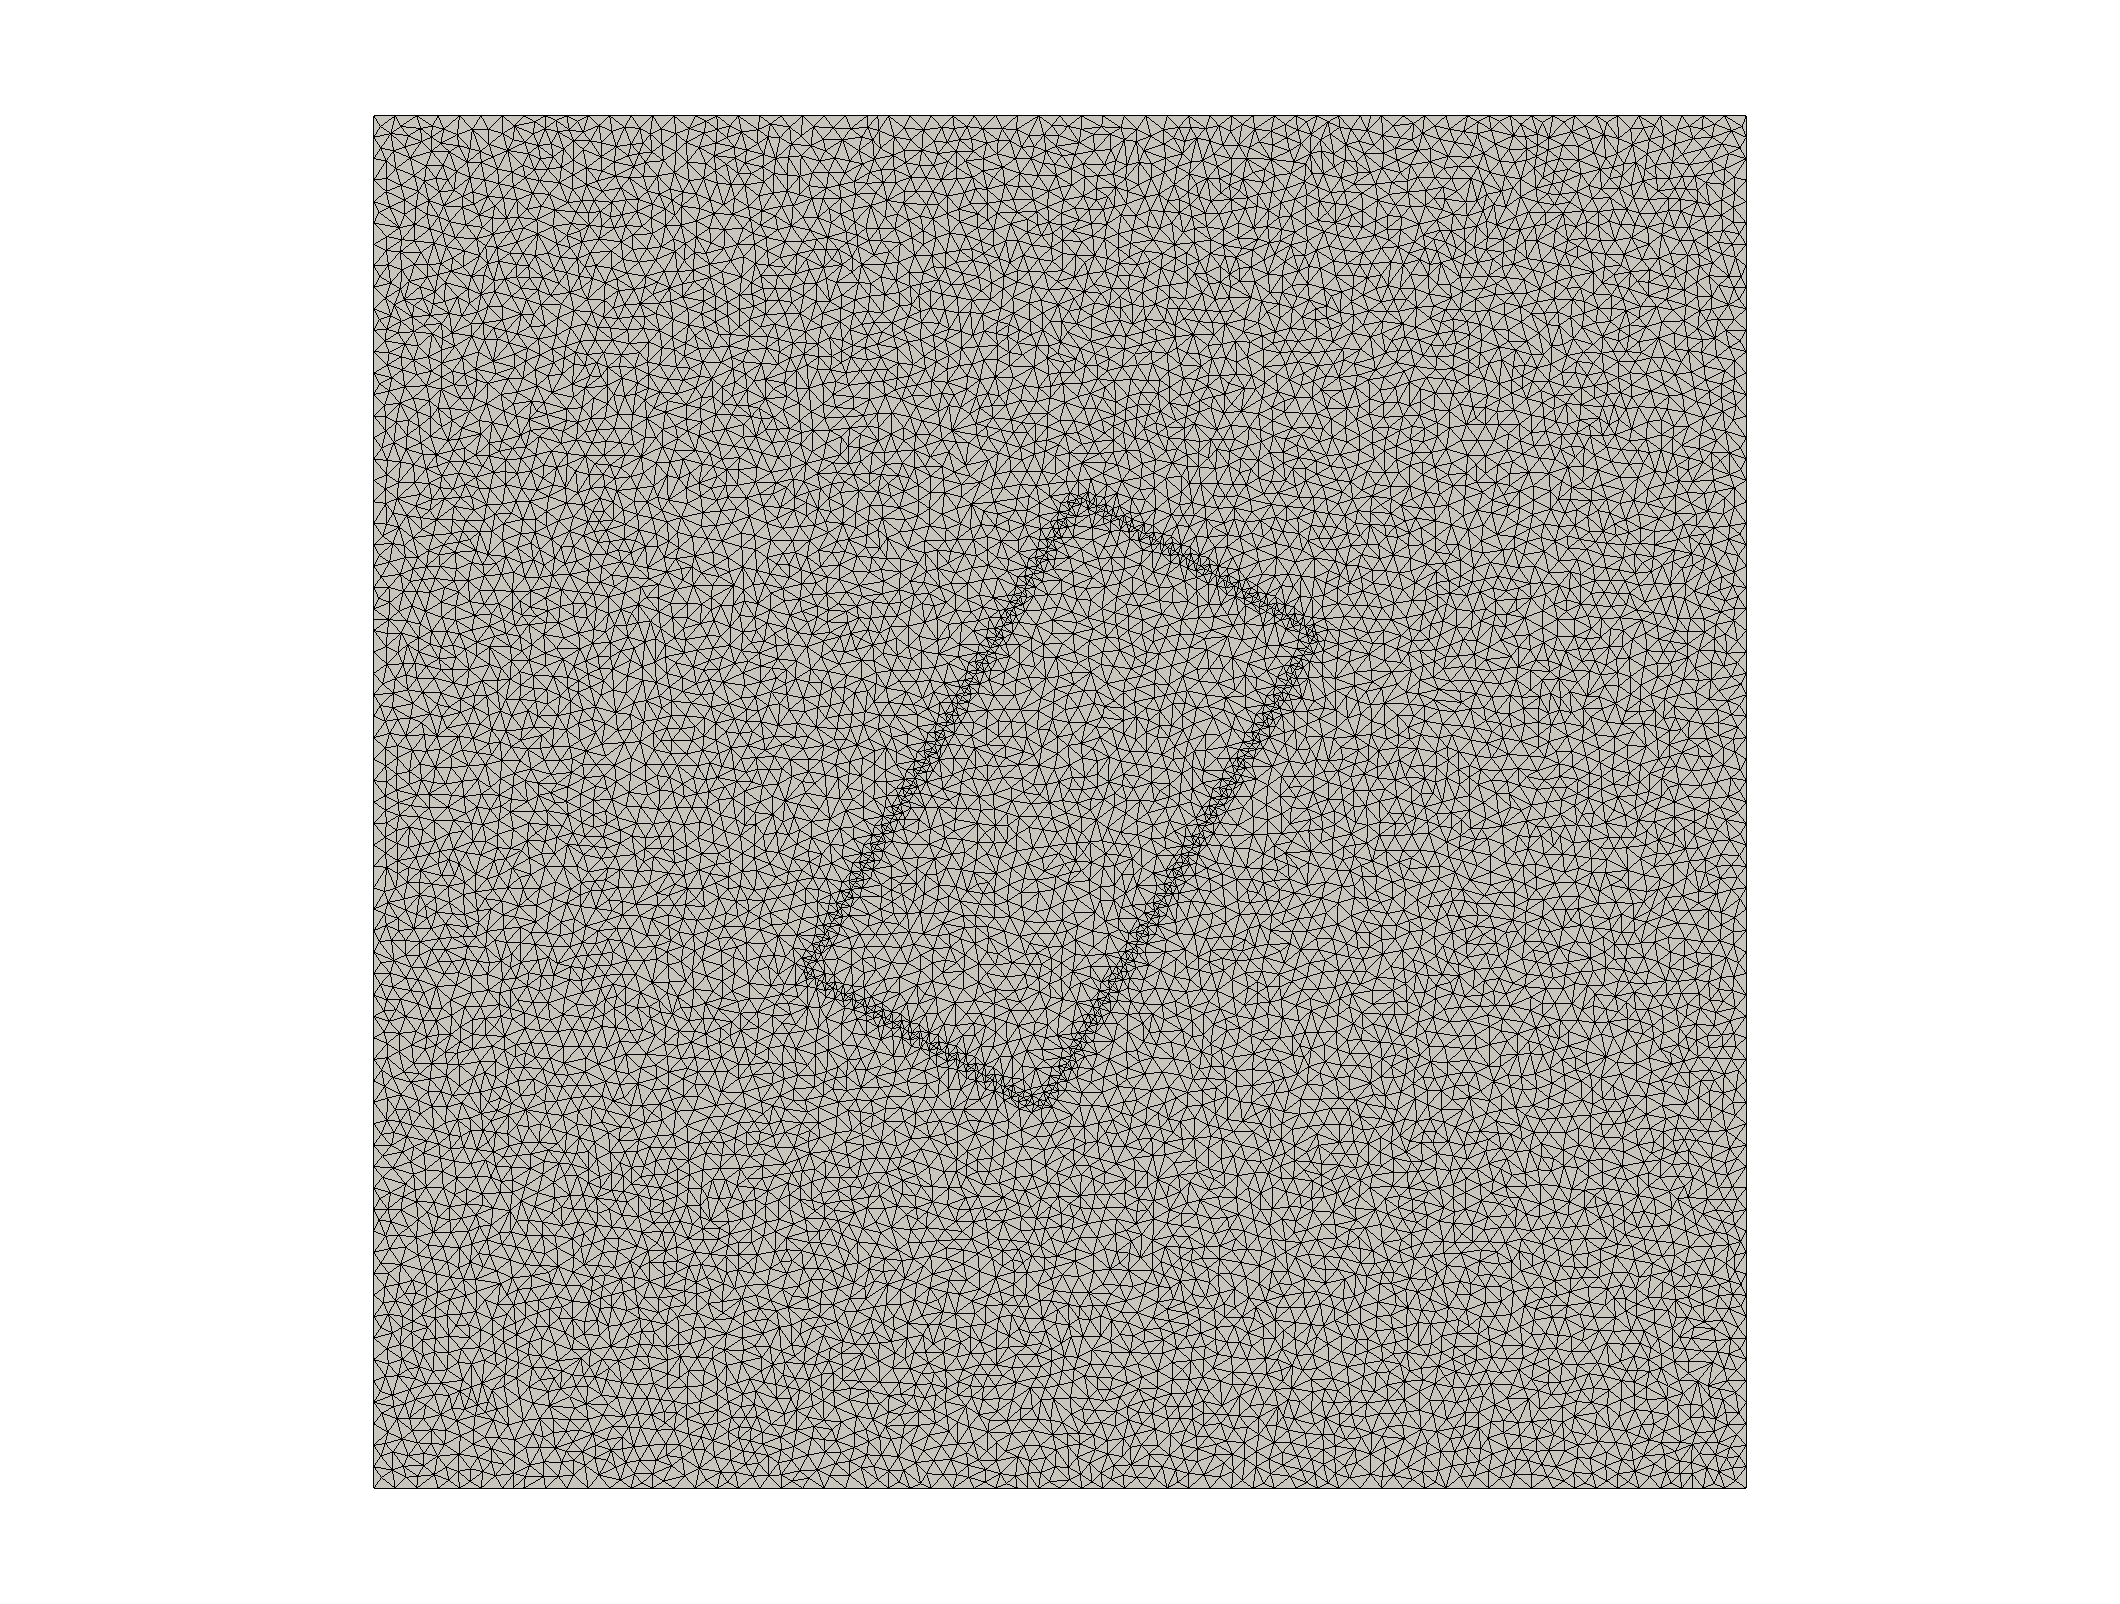
\includegraphics[width=5cm]{python_codes/fieldstone_68/results/case1a/mesh}
\includegraphics[width=5cm]{python_codes/fieldstone_68/results/case1a/fix_uv}
\includegraphics[width=5cm]{python_codes/fieldstone_68/results/case1a/fix_T}\\
{\captionfont Left: mesh composed of 66x60 square elements; 
Middle: where velocity boundary conditions are prescribed;
Right: where temperature boundary conditions are prescribed.}
\end{center}

Except for case 1a, the Stokes equation is solved. It is solved on the whole domain 
but we only care about the solution inside the wedge. The velocity field outside the wedge 
is overwritten by the desired velocity field before the temperature equation is solved.


\begin{center}
\includegraphics[width=5cm]{python_codes/fieldstone_68/results/case1a/vel_zoom}\\
{\captionfont The paper mentions a velocity ramp in section 2.3. While it is not 
always clear how long it is nor why it should or should not be used in combination
with resolution, it nevertheless makes sure that the point at the 'triple junction'
has a zero velocity. Through trial an error I was able to arrive to the conclusion that 
all nodes upstream of this point should too have a zero velocity.} 
\end{center}

The domain is 660x600km. We can easily generate a mesh made of square elements at any resolution 
but we need the bottom of the lithosphere to align with a row of nodes, which limits the 
used resolutions to 66x60 (10km resolution), 132x120 (5km resolution), 264x240 (2.5km resolution)
and 330x300 (2km resolution). Higher resolutions require too much memory. The 330x300 mesh was not 
used for cases 2a and 2b because of the total run time required.

The mesh can be stretched so as to achieve a high(er) resolution in the part of the wedge 
where some measurements are taken:
\begin{center}
\includegraphics[width=7cm]{python_codes/fieldstone_68/images/mesh_stretch}
\includegraphics[width=7cm]{python_codes/fieldstone_68/images/mesh_stretch_zoom}
\end{center}


%..........................................
\subsubsection*{Description of the code}


Crouzeix-Raviart elements are used for the Stokes equations (see Section~\ref{sec:crouzeix-raviart}) 
and $P_2$ elements are used for the temperature. 

The origin of the coordinate system $(x,y)$ is at the bottom left. 
The boundary conditions for the
wedge are no-slip below the overriding plate and constant velocity along the top of the slab. 
The velocity boundary conditions for the boundaries of the wedge are either provided by the Batchelor 
cornerflow solution (case 1b) or based on free inflow/outflow boundaries. 
The velocity field is discontinuous between the slab and the overriding plate which 
effectively mimics the fault representative of the seismogenic zone in subduction zones.

For cases 1a,b,c the Stokes equations and the energy equation are not really coupled: 
the gravity is set to zero, the model is driven by the kinematical boundary conditions 
and the viscosity is constant, so that temperature does not 
influence the Stokes solve. Once the velocity field is obtained it is used 
in the energy equation to compute the steady state temperature field. 

For cases 2a,b the viscosity of the mantle 
wedge is temperature (and strain rate) dependent so that the coupling of the PDEs 
requires nonlinear iterations. These are as follows:
\begin{enumerate}
\item set $\vec{\upnu}_{old}$=0, $T_{old}=0$ at all mesh nodes.
\item Solve Stokes equation with $\eta(T_{old},\dot{\varepsilon}_{old})$ (if iter=0, use $\eta=10^{21}$ for the whole domain).
\item Relax the velocity solution: $\vec\upnu = relax \cdot \vec{\upnu} + (1-relax)\cdot \vec{\upnu}_{old}$
\item Solve for temperature 
\item Relax the temperature solution: $T=relax \cdot T + (1-relax) \cdot T_{old}$
\item Check for convergence. If $\|\vec\upnu-\vec\upnu_{old}\|_2 < tol \| \vec\upnu + \vec\upnu_{old}  \|_2$ i
and $\|T-T_{old}\|_2 < tol \| T + T_{old}  \|_2$ then exit, 
otherwise: $T_{old} \leftarrow T$, $ \vec\upnu \leftarrow \vec\upnu_{old} $. iter+=1. Go back to 2. 
\end{enumerate}

The $relax$ parameter should obviously be between 0 and 1 and set to 0.8. 
To compare model results each
group contributed the temperature field as discrete values $T_{ij}$ on
an equidistant grid with 6 km spacing, which is a 111x101 matrix
stored row-wise starting in the top left corner. 

\begin{center}
\includegraphics[width=5cm]{python_codes/fieldstone_68/images/grid1}
\includegraphics[width=5cm]{python_codes/fieldstone_68/images/grid2}\\
{\captionfont Measuring grid made of 110x100 points.}
\end{center}

From this grid we have extracted the following measurements for direct comparison:
\begin{itemize}
\item the temperature $T_{11,11}$ which is at coordinates (60, 60 km) and
just down-stream from the corner point.
\item the L2 norm of the slab–wedge interface temperature between
0 and 210 km depth defined by
\[
T_{slab} = \sqrt{\frac{1}{36} \sum_{i=1}^{36} T_{ii}^2  }
\]
\item 
the L2 norm of the temperature in the triangular part of the
tip of the wedge, between 54 and 120 km depth:
\[
T_{wedge} = \sqrt{ \frac{1}{78} \sum_{i=10}^{21} \sum_{j=10}^i T_{ij}^2   }
\]
\end{itemize}

\begin{center}
\includegraphics[width=5cm]{python_codes/fieldstone_68/images/grid3}
\includegraphics[width=5cm]{python_codes/fieldstone_68/images/grid4}
\includegraphics[width=5cm]{python_codes/fieldstone_68/images/grid5}\\
{\captionfont The black dots indicate the different types of reported quantities in the paper.}
\end{center}


In order to interpolate temperature on this grid, we need to find out in which 
triangle each point of the grid lies. When the mesh is made of irregular triangles, 
it is a rather costly algorithm. When the mesh is as described above, we first 
determine in which square element  a point lies and then in which of the 
two triangles. 

In general, in order to determine whether a point is inside a triangle, we assume that 
the reduced coordinates $r,s$ exist and satisfy the following 
relationships:
\begin{eqnarray}
x &=& N_1(r,s) x_1 + N_2(r,s) x_2 + N_3(r,s) x_3 \nn\\  
y &=& N_1(r,s) y_1 + N_2(r,s) y_2 + N_3(r,s) y_3 \nn
\end{eqnarray}
where $N_i$ are the linear basis functions inside a triangle, see Section~\ref{ss:p1}.

We also have the property that $N_1+N_2+N_3=1$ everywhere inside the element, so that 
we now have a system of 3 equations for our three unknowns $N_1$, $N_2$ and $N_3$ (having
obtained these, we can later easily find $r$ and $s$).
We must then solve:
\begin{eqnarray}
x &=& N_1 x_1 + N_2 x_2 + N_3 x_3 \nn\\  
y &=& N_1 y_1 + N_2 y_2 + N_3 y_3 \nn\\
0 &=& N_1+N_2+N_3 \nn
\end{eqnarray}
which yields
\[
N_1=\frac{(y_2 - y_3)(x - x_3) + (x_3 - x_2)(y - y_3)}{(y_2 - y_3)(x_1 - x_3) + (x_3 - x_2)(y_1 - y_3)}
\qquad
N_2=\frac{(y_3 - y_1)(x - x_3) + (x_1 - x_3)(y - y_3)}{(y_2 - y_3)(x_1 - x_3) + (x_3 - x_2)(y_1 - y_3)}
\qquad
N_3=1-a-b
\]
and then $r=N_2$ and $s=N_3$

To these measurements I have also added the average temperature over the domain 
\[
T_{avrg} = \frac{1}{L_xL_y}\iint T(x,y) dx dy,
\]
the root mean square velocity in the wedge
\[
v_{rms} = \sqrt{  \frac{1}{A_{wedge}} \iint_{wedge} (u^2+v^2) dx dy    },
\]
and the temperature at the top of the slab (line $y=L_y-x$).



\newpage
%------------------------------------------------------------
\subsubsection*{Results - Case 1a} 

\begin{center}
\includegraphics[width=7cm]{python_codes/fieldstone_68/results/case1a/Tcorner}
\includegraphics[width=7cm]{python_codes/fieldstone_68/results/case1a/Twedge}\\
\includegraphics[width=7cm]{python_codes/fieldstone_68/results/case1a/Tslab}
\includegraphics[width=7cm]{python_codes/fieldstone_68/results/case1a/Tavrg}\\
\includegraphics[width=7cm]{python_codes/fieldstone_68/results/case1a/tempdiag}\\
{\captionfont Dashed lines correspond to values reported in Table 2 of \cite{vack08}.
Lines correspond to values communicated to us by P. van Keken.}
\end{center}

\begin{center}
\includegraphics[width=6.7cm]{python_codes/fieldstone_68/results/case1a/vel_1a}
\includegraphics[width=6.7cm]{python_codes/fieldstone_68/results/case1a/T_1a}
\end{center}

\begin{center}
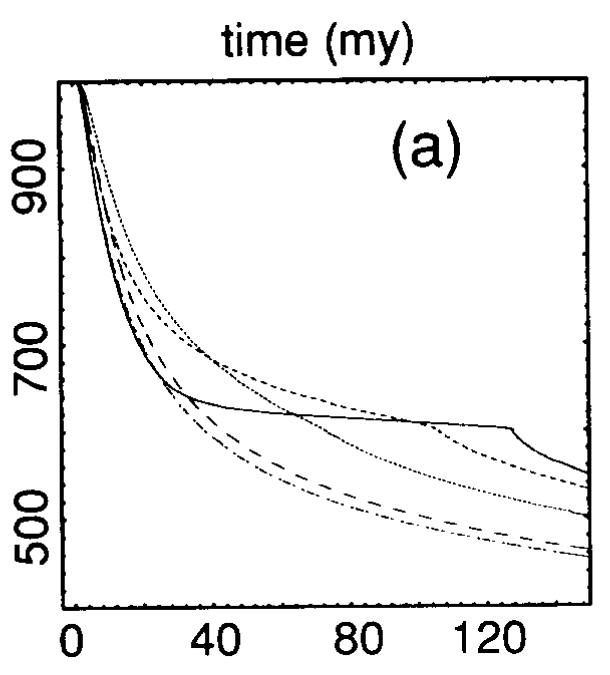
\includegraphics[width=9cm]{python_codes/fieldstone_68/images/fig2}\\
{\captionfont Taken from \cite{vack08}. Temperature prediction for case 1a. 
The bold lines indicate the top of the slab and base of the overriding plate. 
(b) Close up of the top left part of the model.}
\end{center}


\newpage
%----------------------------
\subsubsection*{Results - Case 1b}

\begin{center}
\includegraphics[width=7cm]{python_codes/fieldstone_68/results/case1b/Tcorner}
\includegraphics[width=7cm]{python_codes/fieldstone_68/results/case1b/Twedge}\\
\includegraphics[width=7cm]{python_codes/fieldstone_68/results/case1b/Tslab}
\includegraphics[width=7cm]{python_codes/fieldstone_68/results/case1b/Tavrg}\\
\includegraphics[width=7cm]{python_codes/fieldstone_68/results/case1b/tempdiag}\\
{\captionfont Dashed lines correspond to values reported in Table 2 of \cite{vack08}.
Lines correspond to values communicated to us by P. van Keken.}
\end{center}

\begin{center}
\includegraphics[width=7cm]{python_codes/fieldstone_68/results/case1b/vel_1b}
\includegraphics[width=7cm]{python_codes/fieldstone_68/results/case1b/T_1b}
\end{center}



\newpage
%----------------------------
\subsubsection*{Results - Case 1c}

\begin{center}
\includegraphics[width=7cm]{python_codes/fieldstone_68/results/case1c/Tcorner}
\includegraphics[width=7cm]{python_codes/fieldstone_68/results/case1c/Twedge}\\
\includegraphics[width=7cm]{python_codes/fieldstone_68/results/case1c/Tslab}
\includegraphics[width=7cm]{python_codes/fieldstone_68/results/case1c/Tavrg}\\
\includegraphics[width=7cm]{python_codes/fieldstone_68/results/case1c/tempdiag}\\
{\captionfont Dashed lines correspond to values reported in Table 2 of \cite{vack08}.
Lines correspond to values communicated to us by P. van Keken.}
\end{center}

\begin{center}
\includegraphics[width=7cm]{python_codes/fieldstone_68/results/case1c/vel}
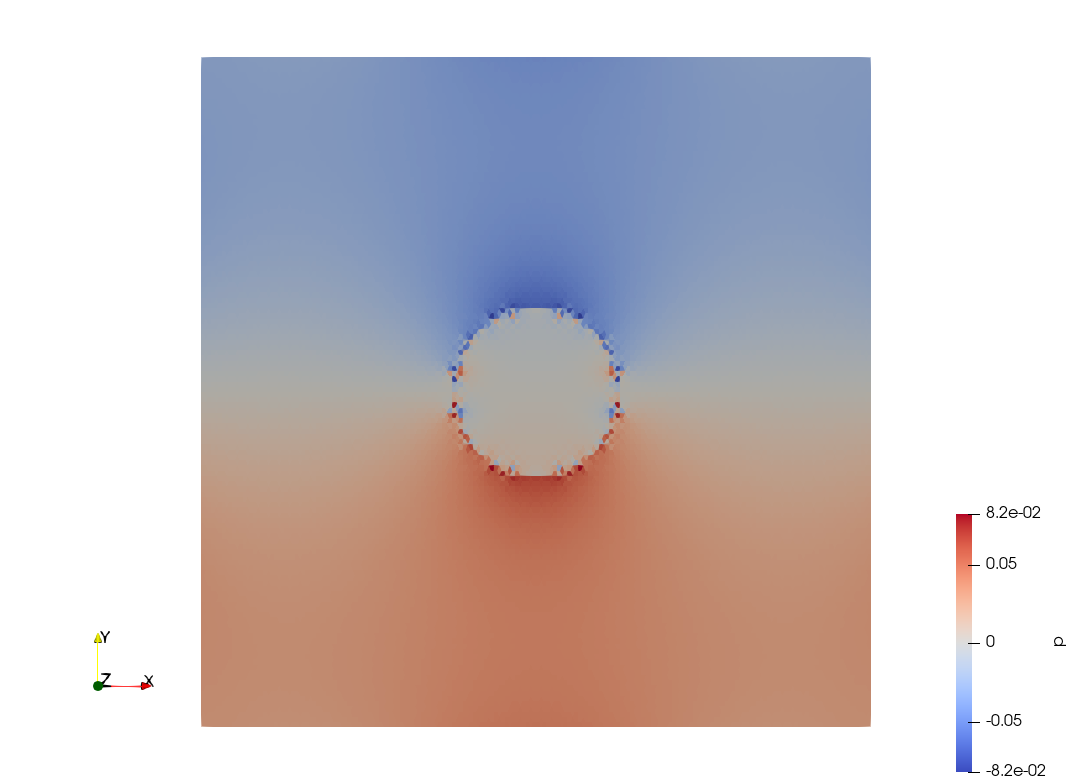
\includegraphics[width=7cm]{python_codes/fieldstone_68/results/case1c/p}\\
\includegraphics[width=7cm]{python_codes/fieldstone_68/results/case1c/T}
\includegraphics[width=7cm]{python_codes/fieldstone_68/results/case1c/T_zoom}
\end{center}

We see that stretching the mesh does not really work since it makes the mesh coarser in the rest of the wedge and therefore 
alter the global solution.

\newpage
%----------------------------
\subsubsection*{Results - Case 2a}

\begin{center}
\includegraphics[width=7cm]{python_codes/fieldstone_68/results/case2a/Tcorner}
\includegraphics[width=7cm]{python_codes/fieldstone_68/results/case2a/Twedge}\\
\includegraphics[width=7cm]{python_codes/fieldstone_68/results/case2a/Tslab}
\includegraphics[width=7cm]{python_codes/fieldstone_68/results/case2a/Tavrg}\\
\includegraphics[width=7cm]{python_codes/fieldstone_68/results/case2a/tempdiag}\\
{\captionfont Dashed lines correspond to values reported in Table 3 of \cite{vack08}.
Lines correspond to values communicated to us by P. van Keken.}
\end{center}

\begin{center}
\includegraphics[width=7cm]{python_codes/fieldstone_68/results/case2a/vel}
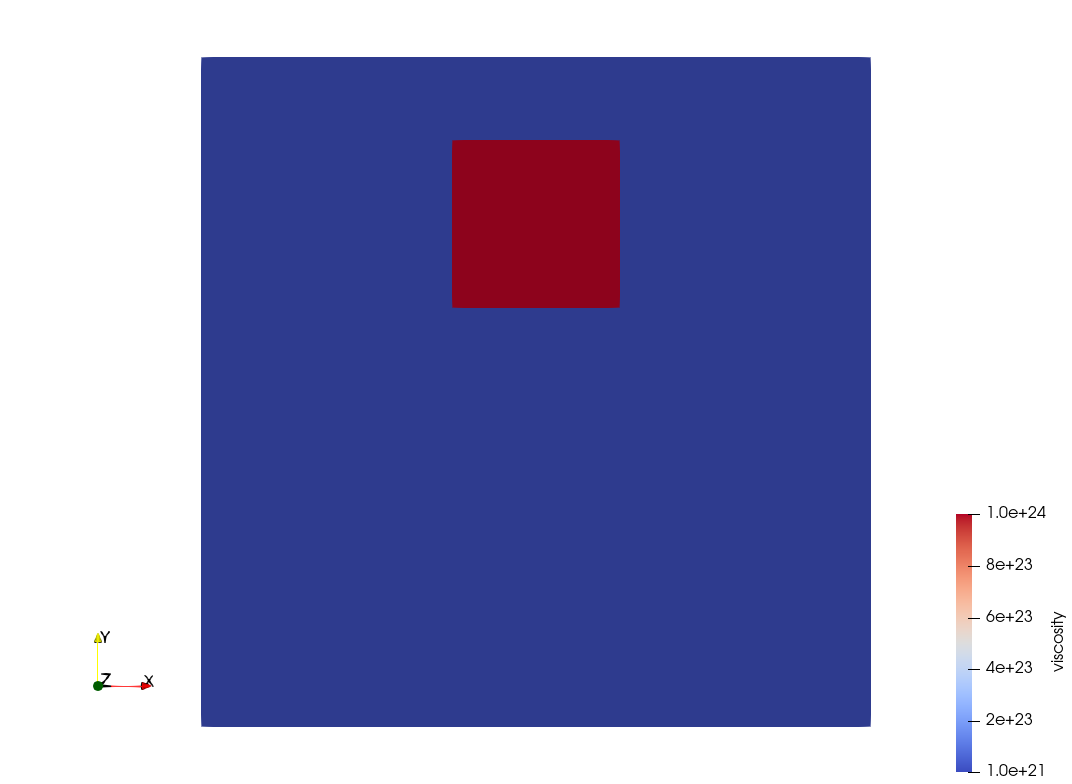
\includegraphics[width=7cm]{python_codes/fieldstone_68/results/case2a/eta}\\
\includegraphics[width=7cm]{python_codes/fieldstone_68/results/case2a/T}
\includegraphics[width=7cm]{python_codes/fieldstone_68/results/case2a/T_zoom}
\end{center}

\begin{center}
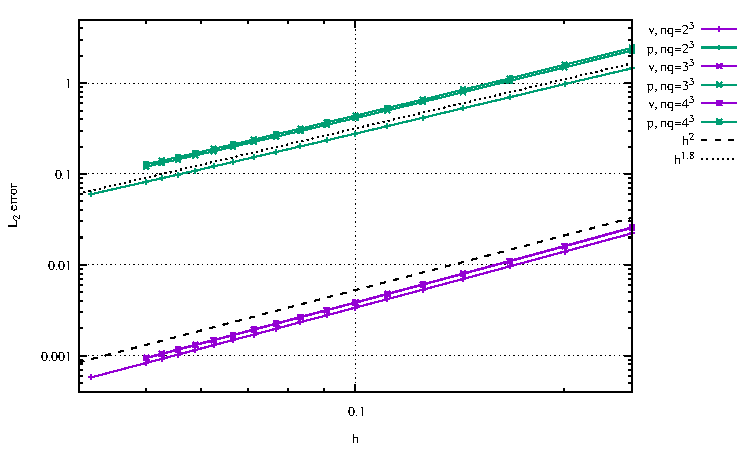
\includegraphics[width=7cm]{python_codes/fieldstone_68/results/case2a/conv.pdf}
\includegraphics[width=7cm]{python_codes/fieldstone_68/results/case2a/stats_Tcorner.pdf}\\
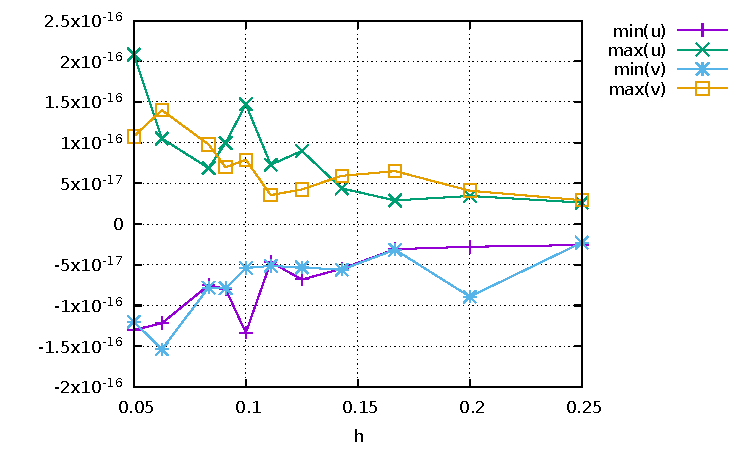
\includegraphics[width=7cm]{python_codes/fieldstone_68/results/case2a/stats_uv.pdf}
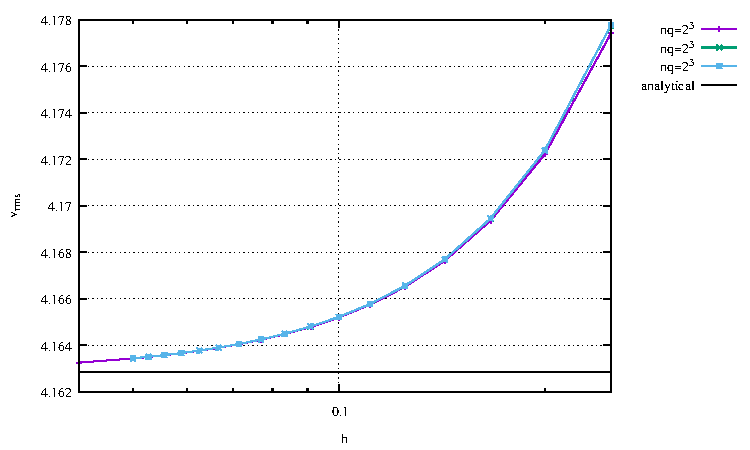
\includegraphics[width=7cm]{python_codes/fieldstone_68/results/case2a/vrms.pdf}
\end{center}


\begin{center}
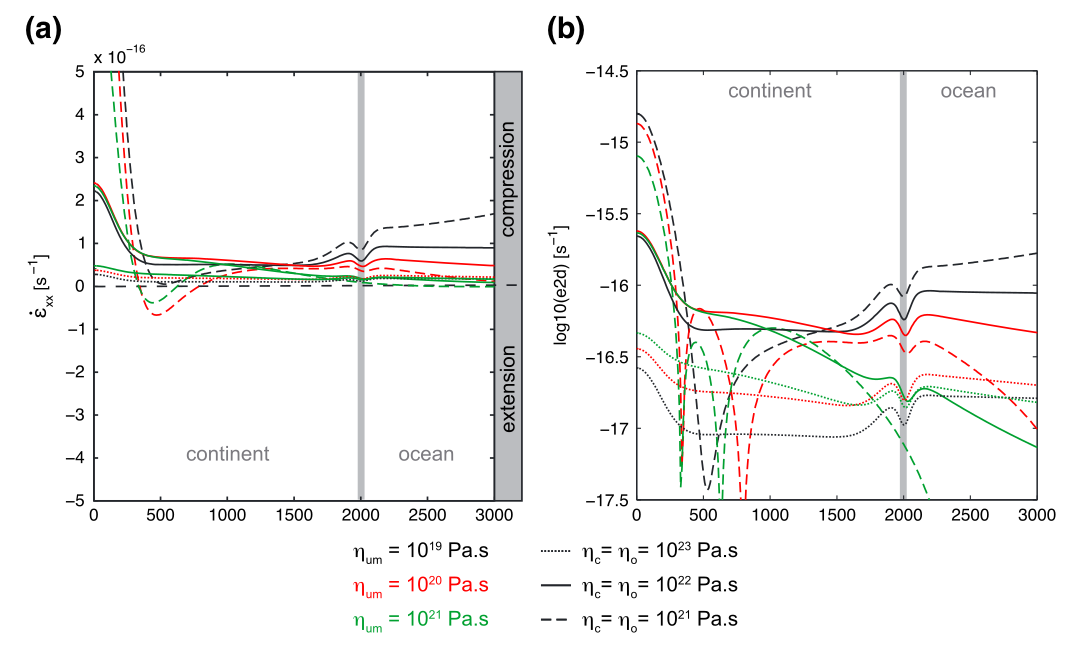
\includegraphics[width=5cm]{python_codes/fieldstone_68/images/fig4}\\
{\captionfont Taken from \cite{vack08}. 
(a) Temperature prediction for case 2a with olivine diffusion creep in 
the mantle wedge. (b) Close up of the top left part of the model, as in Fig. 2b.}
\end{center}

\newpage
%----------------------------
\subsubsection*{Results - Case 2b}

\begin{center}
\includegraphics[width=7cm]{python_codes/fieldstone_68/results/case2b/Tcorner}
\includegraphics[width=7cm]{python_codes/fieldstone_68/results/case2b/Twedge}\\
\includegraphics[width=7cm]{python_codes/fieldstone_68/results/case2b/Tslab}
\includegraphics[width=7cm]{python_codes/fieldstone_68/results/case2b/Tavrg}\\
\includegraphics[width=7cm]{python_codes/fieldstone_68/results/case2b/tempdiag}\\
{\captionfont Dashed lines correspond to values reported in Table 3 of \cite{vack08}.
Lines correspond to values communicated to us by P. van Keken.}
\end{center}

\begin{center}
\includegraphics[width=7cm]{python_codes/fieldstone_68/results/case2b/vel}
\includegraphics[width=7cm]{python_codes/fieldstone_68/results/case2b/eta}\\
\includegraphics[width=7cm]{python_codes/fieldstone_68/results/case2b/T}
\includegraphics[width=7cm]{python_codes/fieldstone_68/results/case2b/T_zoom}
\end{center}

\begin{center}
\includegraphics[width=7cm]{python_codes/fieldstone_68/results/case2b/conv.pdf}
\includegraphics[width=7cm]{python_codes/fieldstone_68/results/case2b/stats_Tcorner.pdf}\\
\includegraphics[width=7cm]{python_codes/fieldstone_68/results/case2b/stats_uv.pdf}
\includegraphics[width=7cm]{python_codes/fieldstone_68/results/case2b/vrms.pdf}
\end{center}

\begin{center}
\includegraphics[width=5cm]{python_codes/fieldstone_68/images/fig4c}\\
{\captionfont Taken from \cite{vack08}. 
Close up of the model with olivine dislocation creep in the mantle wedge.}
\end{center}




%\begin{landscape}
%\includegraphics[width=11.5cm]{python_codes/fieldstone_68/images/fig3}
%\includegraphics[width=11.5cm]{python_codes/fieldstone_68/results/van_keken_2008_fig3.jpg}\\
%{\captionfont Left: Taken from \cite{vack08}. 
%Predictions for selected thermal properties for the isoviscous benchmark cases 1a 
%(frames a-c), 1b (d-f) and 1c (g-i). The quantities represent a spot measurement at
%the slab–wedge interface at 60 km depth (frames a, d, g), the average temperature 
%along the slab–wedge interface from 0 to 210 km depth (frames b, e, h), and the
%average temperature in a triangular portion of the wedge (frames c, f, i). 
%The averages are computed with an L2 norm from an equidistant grid with 6 km spacing.
%Right: recreated figure with additional fieldstone results in yellow.
%}
%\end{landscape}

 
%\newpage
%----------------------------
%\paragraph{Cases 2a}.

%\begin{center}
%\includegraphics[width=5.cm]{python_codes/fieldstone_68/results/case2a/T}
%\includegraphics[width=5.cm]{python_codes/fieldstone_68/results/case2a/u}
%\includegraphics[width=5.cm]{python_codes/fieldstone_68/results/case2a/v}\\
%\includegraphics[width=5.cm]{python_codes/fieldstone_68/results/case2a/vel}
%\includegraphics[width=5.cm]{python_codes/fieldstone_68/results/case2a/e}
%\includegraphics[width=5.cm]{python_codes/fieldstone_68/results/case2a/eta}\\
%{\captionfont Case 2a. 4km resolution}
%\end{center}

%\begin{center}
%\includegraphics[width=10cm]{python_codes/fieldstone_68/results/case2a/conv.pdf}\\
%{\captionfont obtained with $tol=10^{-4}$}
%\end{center}

%\begin{center}
%\includegraphics[width=3.74cm]{python_codes/fieldstone_68/results/case2a/eta0000}
%\includegraphics[width=3.74cm]{python_codes/fieldstone_68/results/case2a/eta0009}
%\includegraphics[width=3.74cm]{python_codes/fieldstone_68/results/case2a/eta0019}
%\includegraphics[width=3.74cm]{python_codes/fieldstone_68/results/case2a/eta0028}\\
%\includegraphics[width=3.74cm]{python_codes/fieldstone_68/results/case2a/T0000}
%\includegraphics[width=3.74cm]{python_codes/fieldstone_68/results/case2a/T0009}
%\includegraphics[width=3.74cm]{python_codes/fieldstone_68/results/case2a/T0019}
%\includegraphics[width=3.74cm]{python_codes/fieldstone_68/results/case2a/T0028}\\
%{\captionfont Quadrature points. Top row: viscosity; Bottom row: temperature.
%from left to right: iteration 0,9,19,28.}
%\end{center}


%_______________________
%\paragraph{Cases 2b}.

%\begin{center}
%\includegraphics[width=10cm]{python_codes/fieldstone_68/results/case2b/conv.pdf}\\
%{\captionfont obtained with $tol=10^{-4}$}
%\end{center}
%
%\begin{center}
%\includegraphics[width=5.cm]{python_codes/fieldstone_68/results/case2b/T}
%\includegraphics[width=5.cm]{python_codes/fieldstone_68/results/case2b/u}
%\includegraphics[width=5.cm]{python_codes/fieldstone_68/results/case2b/v}\\
%\includegraphics[width=5.cm]{python_codes/fieldstone_68/results/case2b/vel}
%\includegraphics[width=5.cm]{python_codes/fieldstone_68/results/case2b/e}
%\includegraphics[width=5.cm]{python_codes/fieldstone_68/results/case2b/eta}\\
%{\captionfont Case 2a. 4km resolution}
%\end{center}

%\begin{landscape}
%\includegraphics[width=8cm]{python_codes/fieldstone_68/images/fig5}
% + Iris figure soon
%\end{landscape}




